\section{Doppelbelichtung}
\subsection{Versuchsbeschreibung}

Bei der Doppelbelichtungstechnik wird ein Hologramm des zu untersuchenden Objekts aufgenommen. Dabei befindet sich dieses während einer Hälfte der Belichtungszeit im ersten Zustand und wird dann für den Rest der Zeit in den zweiten Zustand gebracht. Man sieht dann im fertigen Hologramm die Interferenz beider Zustände.

In unserem Fall soll das Biegeverhalten von Metallstäben untersucht werden. Diese werden dazu sowohl mit als auch ohne einem ziehenden Gewicht aufgenommen. Aus dem Interferenzmuster können dann die Weglängenunterschiede und somit die Biegung der Stäbe ermittlelt werden. 

\subsection{Durchführung und Auswertung}

Wie beim vorherigen Versuchsteil begründet, verwenden wir den neuen Tisch und haben den in Abb \ref{doppelbelichtung-aufbau} skizzierten Aufbau verwendet. Da der Laser hier deutlich niedriger positioniert war, haben wir ihn zuerst mit zwei Spiegeln (a, b) um einige Zentimeter erhöht. Dann wird der Strahl wieder mit dem Strahlteiler (c) aufgetrennt in einen Objekt- und einen Referenzstrahl. Der Referenzstrahl wird mit einem Spiegel (d) umgelenkt und trifft direkt auf den Film (i). Der Objektstrahl wird über einen weiteren Spiegel (f) umgelenkt, so dass er auf das Objekt (h) fällt. Seine Reflektion am Objekt interferiert dann mit dem Referenzstrahl auf dem Film und liefert das Hologrammbild. Soweit der einfache Teil. Um ein ausreichend großes und homogenes Leuchtfeld zu erreichen, wird der Strahl mit einem Mikroskopobjektiv aufgeweitet und ein Lochfilter in dessen Brennpunkt gebracht. Das Loch, das sog. "`pinhole"', mit einem Durchmesser von ca. $10\mu m$ muss dabei sehr genau justiert werden, was uns große Freude bereitete. Diese Konstruktion soll auch höhere Beugungsordnungen herausfiltern und wird daher Raumfilter genannt. Wir haben sie (e, g) zwischen den letzten Spiegeln und dem Objekt/Film eingebaut. Das Verhältnis von Objekt- zu Referenzstrahl auf dem Film sollte etwa 1:10 bis 1:30 betragen und mit der Photodiode justiert werden. Es stellte sich jedoch heraus, dass diese bei weitem nicht sensitiv genug ist. Wir haben aber den Strahlteiler sowieso so eingestellt das nahezu alle Intensität im Objektstrahl lag, da bei der Reflektion am Objekt große Streuverluste auftreten. 

Wir haben dann ein Bild mit den empfohlenen Einstellungen \cite{versuchsanleitung} aufgenommen und entwickelt, konnten aber im fertigen Bild nichts erkennen. Die angegebene Belichtungszeit von 50s scheint uns die Hauptursache dafür zu sein. Für die weiteren Aufnahmen haben wir dann die folgenden mündlich überlieferten Prozessschritte \cite{lena_christian} verwendet:

\begin{table}[H]
\begin{tabular}{l}
 \toprule
 2 x 5min belichten\\
 2min entwickeln\\
 10s vorwässern\\
 2min wässern\\
 2min bleichen\\
 10s vorwässern\\
 10min wässern (laufend)\\
 1min wässern (Spülmittel) \\
 \bottomrule 
\end{tabular}
\caption{Prozessschritte für die Erstellung von Holographien auf Planfilmstücken}
\end{table}

Mit diesen erhielten wir dann ein gutes Hologramm (Abb. \ref{doppelbelichtung-links}), wobei allerdings der Aluminiumstab kaum beleuchtet war. Für diesen haben wir daher ein weiteres Bild (Abb. \ref{doppelbelichtung-rechts}) mit angepasster Beleuchtung aufgenommen. Unser Maskotchen Heinrich, den wir ebenfalls mit abbilden wollten, kann man leider nicht erkennen. 

\begin{figure}[H]
 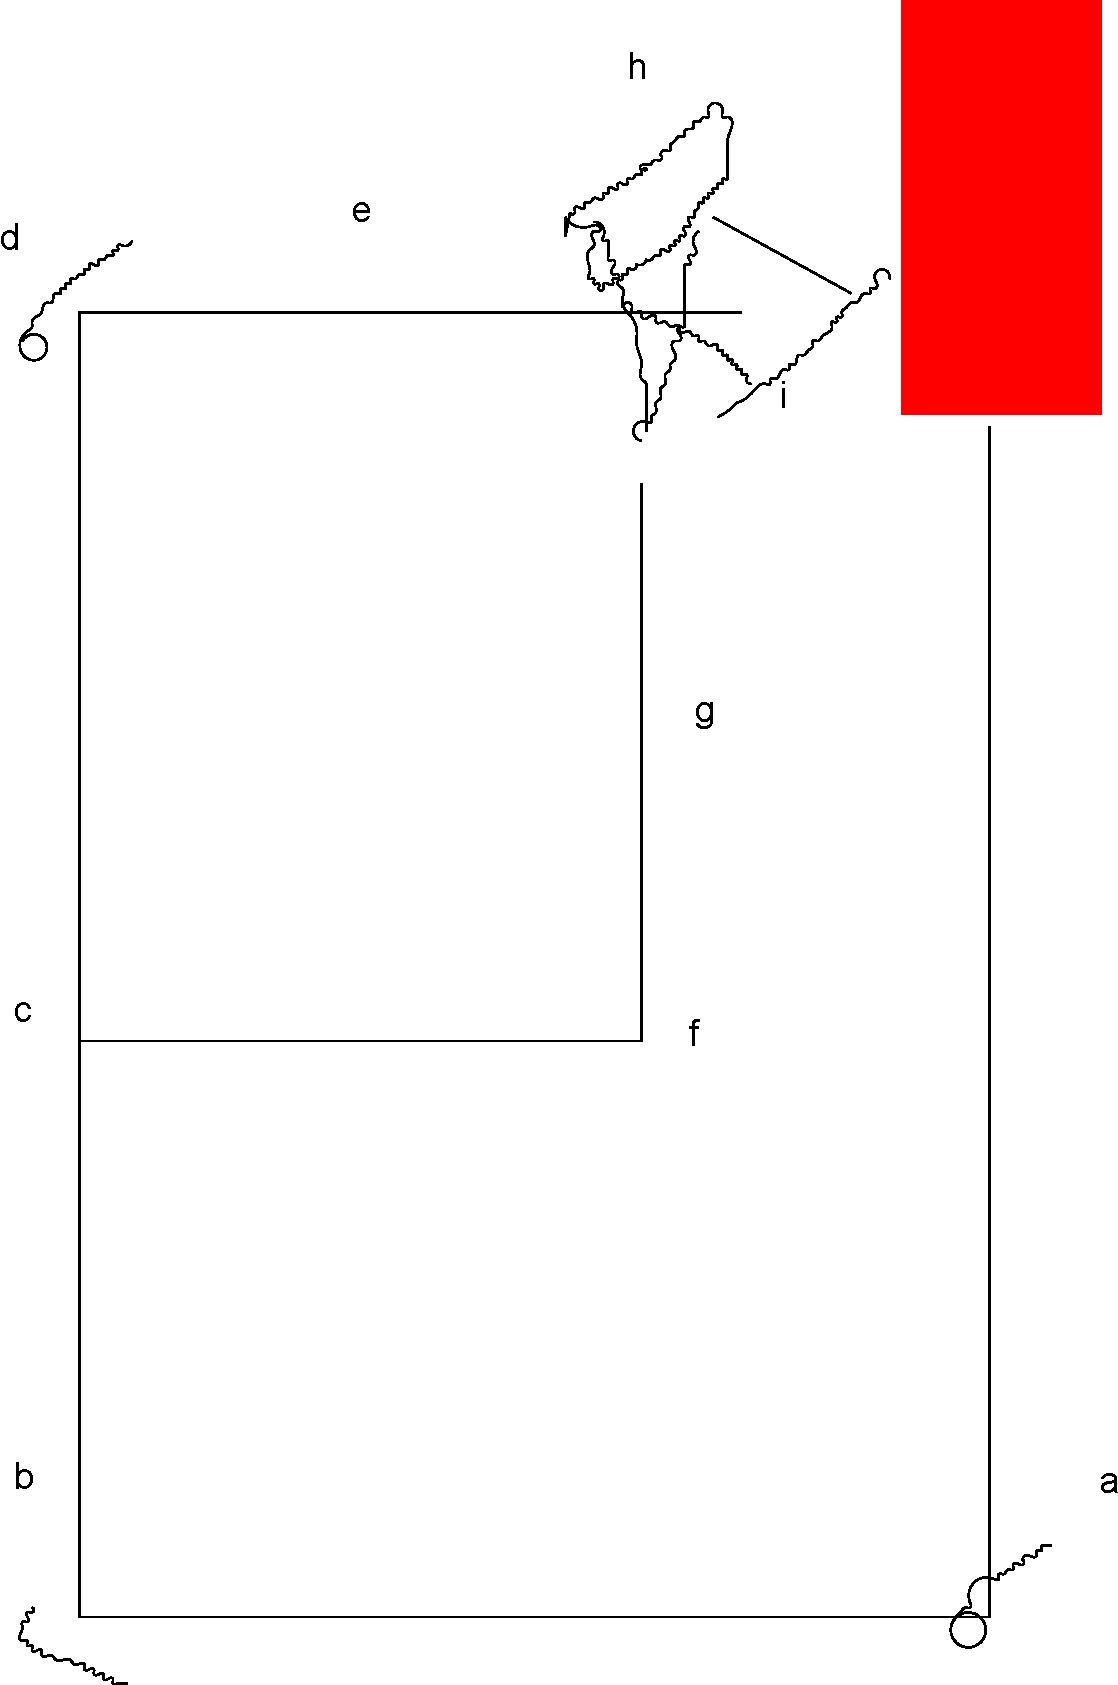
\includegraphics[height=0.5\textheight]{BilderAufbau/doppelbelichtung.pdf}
 \caption{Schematischer Versuchsaufbau für die Doppelbelichtungsholographie}
 \label{doppelbelichtung-aufbau}
\end{figure}


\begin{figure}[H]
 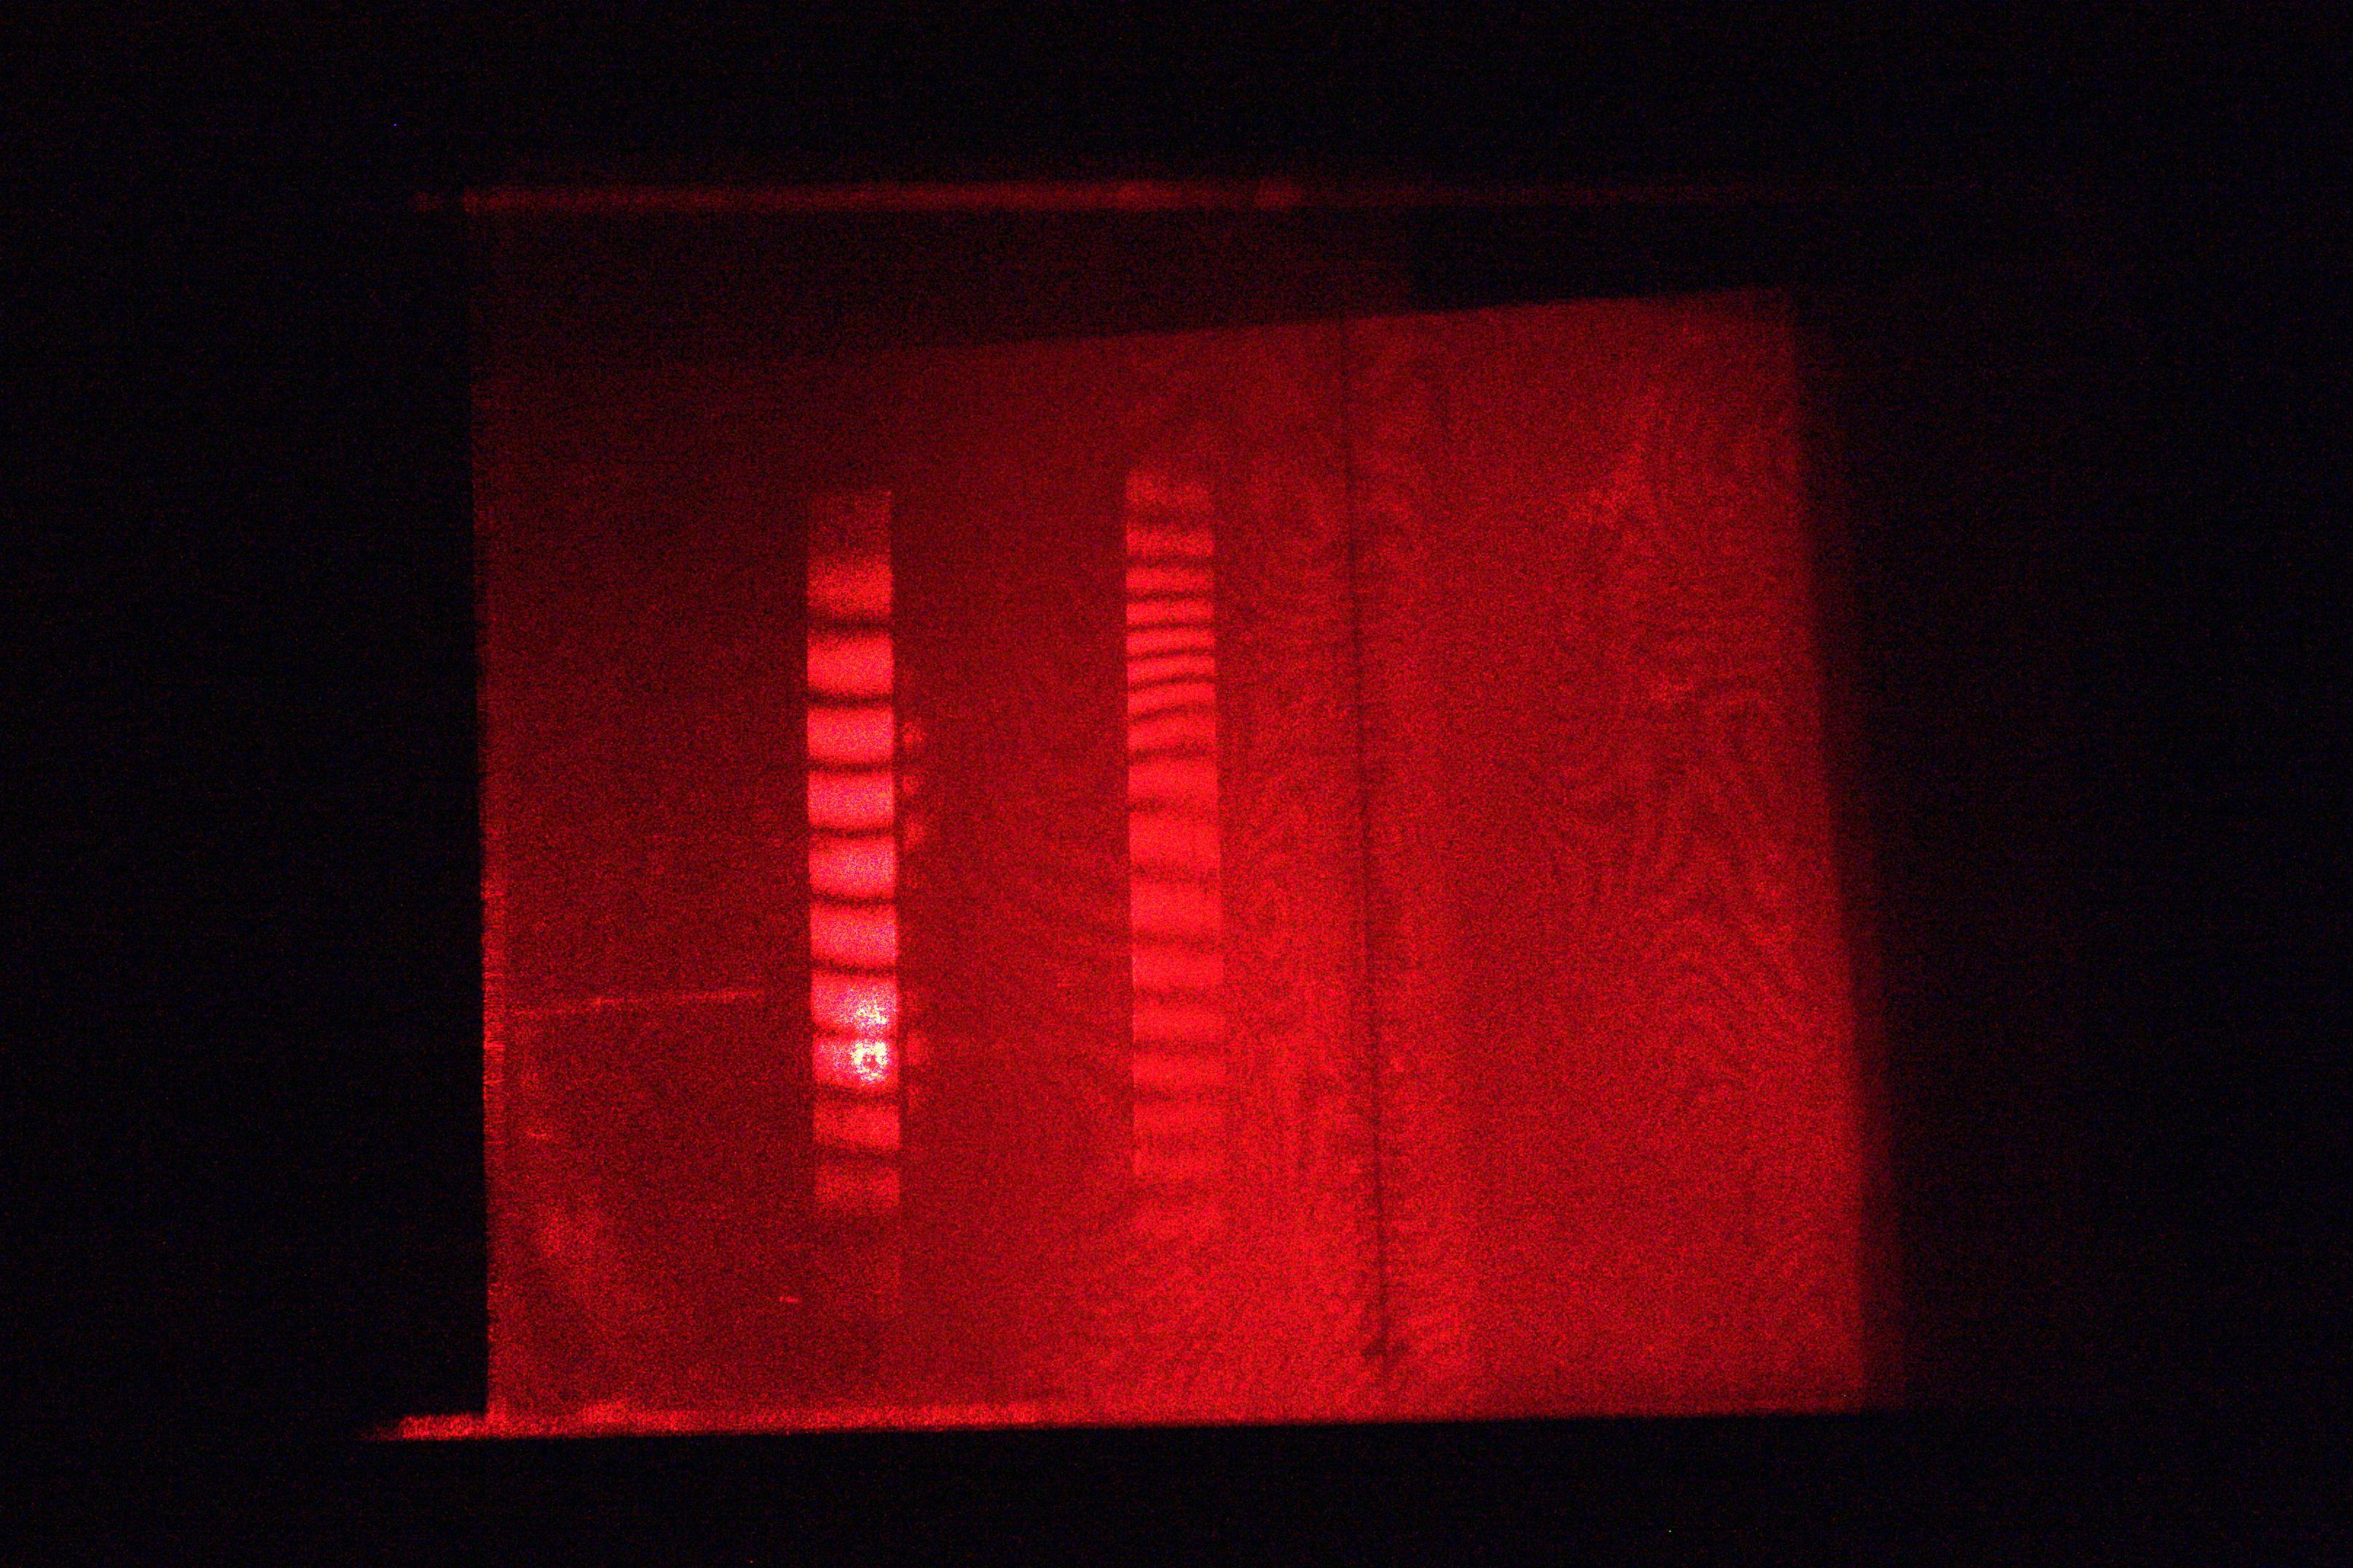
\includegraphics[width=\textwidth]{Photos/IMG_3909.jpg}
 \caption{Hologramm der linken beiden Stäbe}
 \label{doppelbelichtung-links}
\end{figure}


\begin{figure}[ht]
 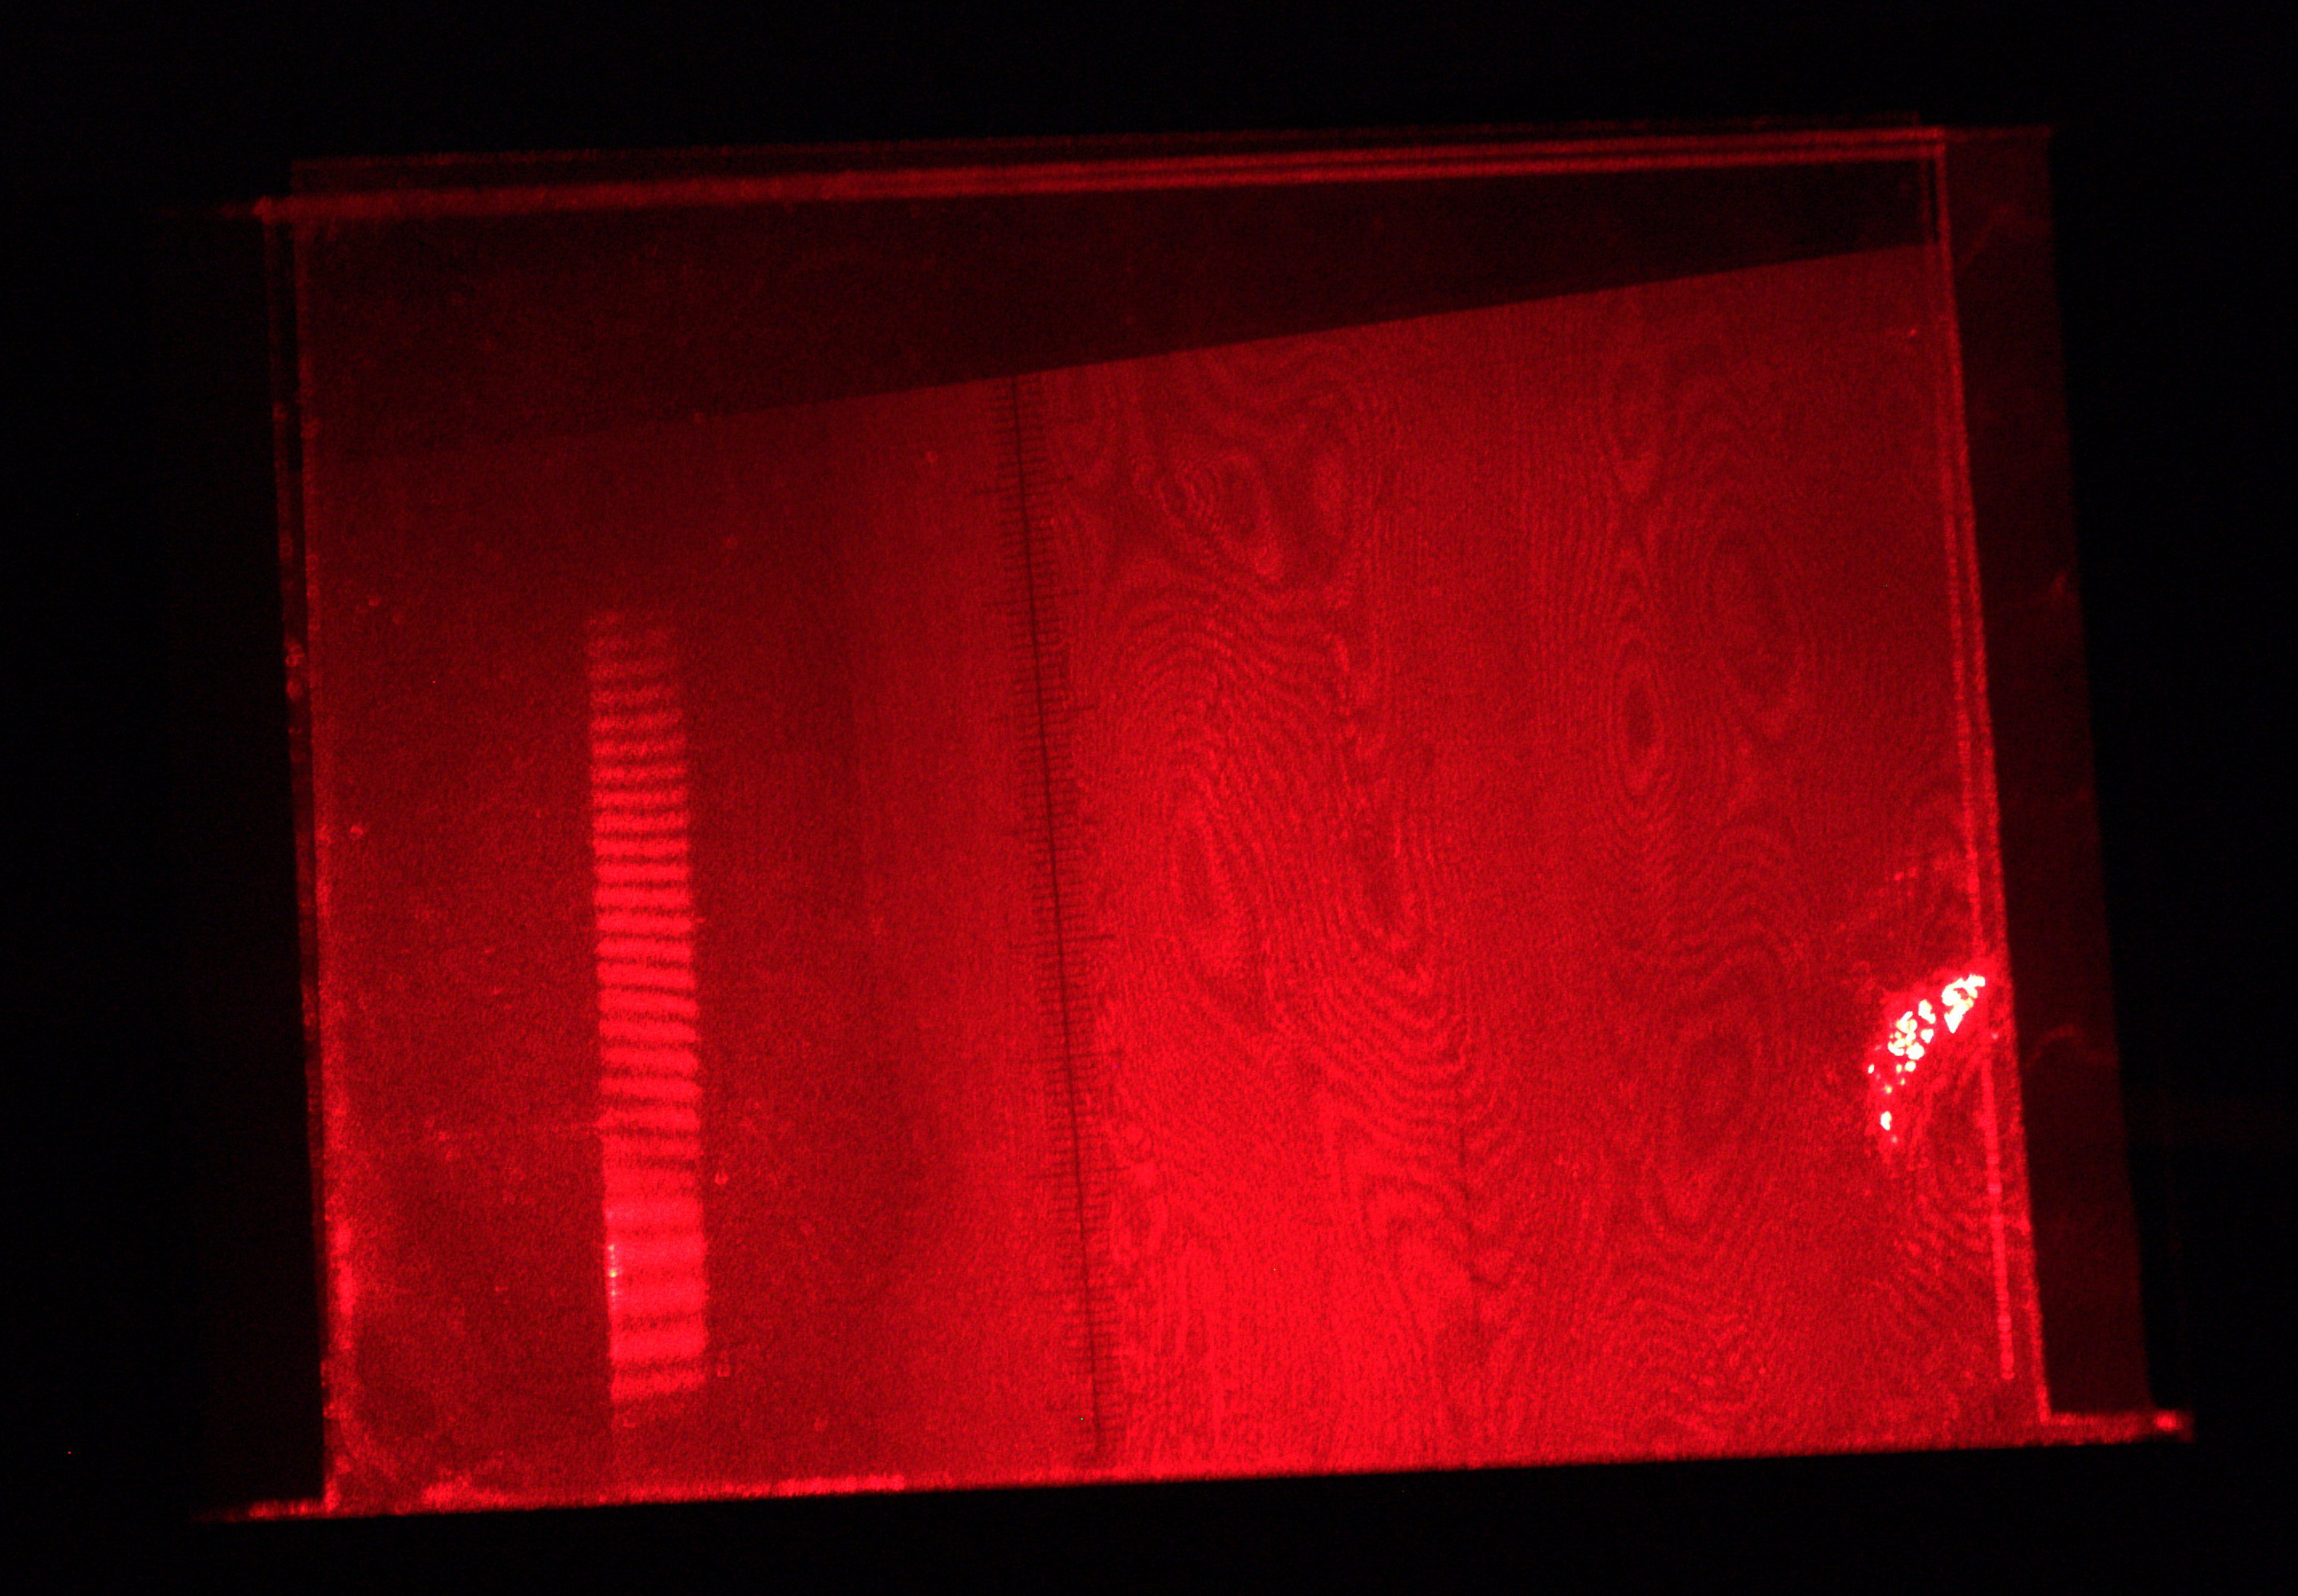
\includegraphics[width=\textwidth]{Photos/IMG_3919.jpg}
 \caption{Hologramm des rechten Stabes}
 \label{doppelbelichtung-rechts}
\end{figure}

\begin{figure}[ht]
 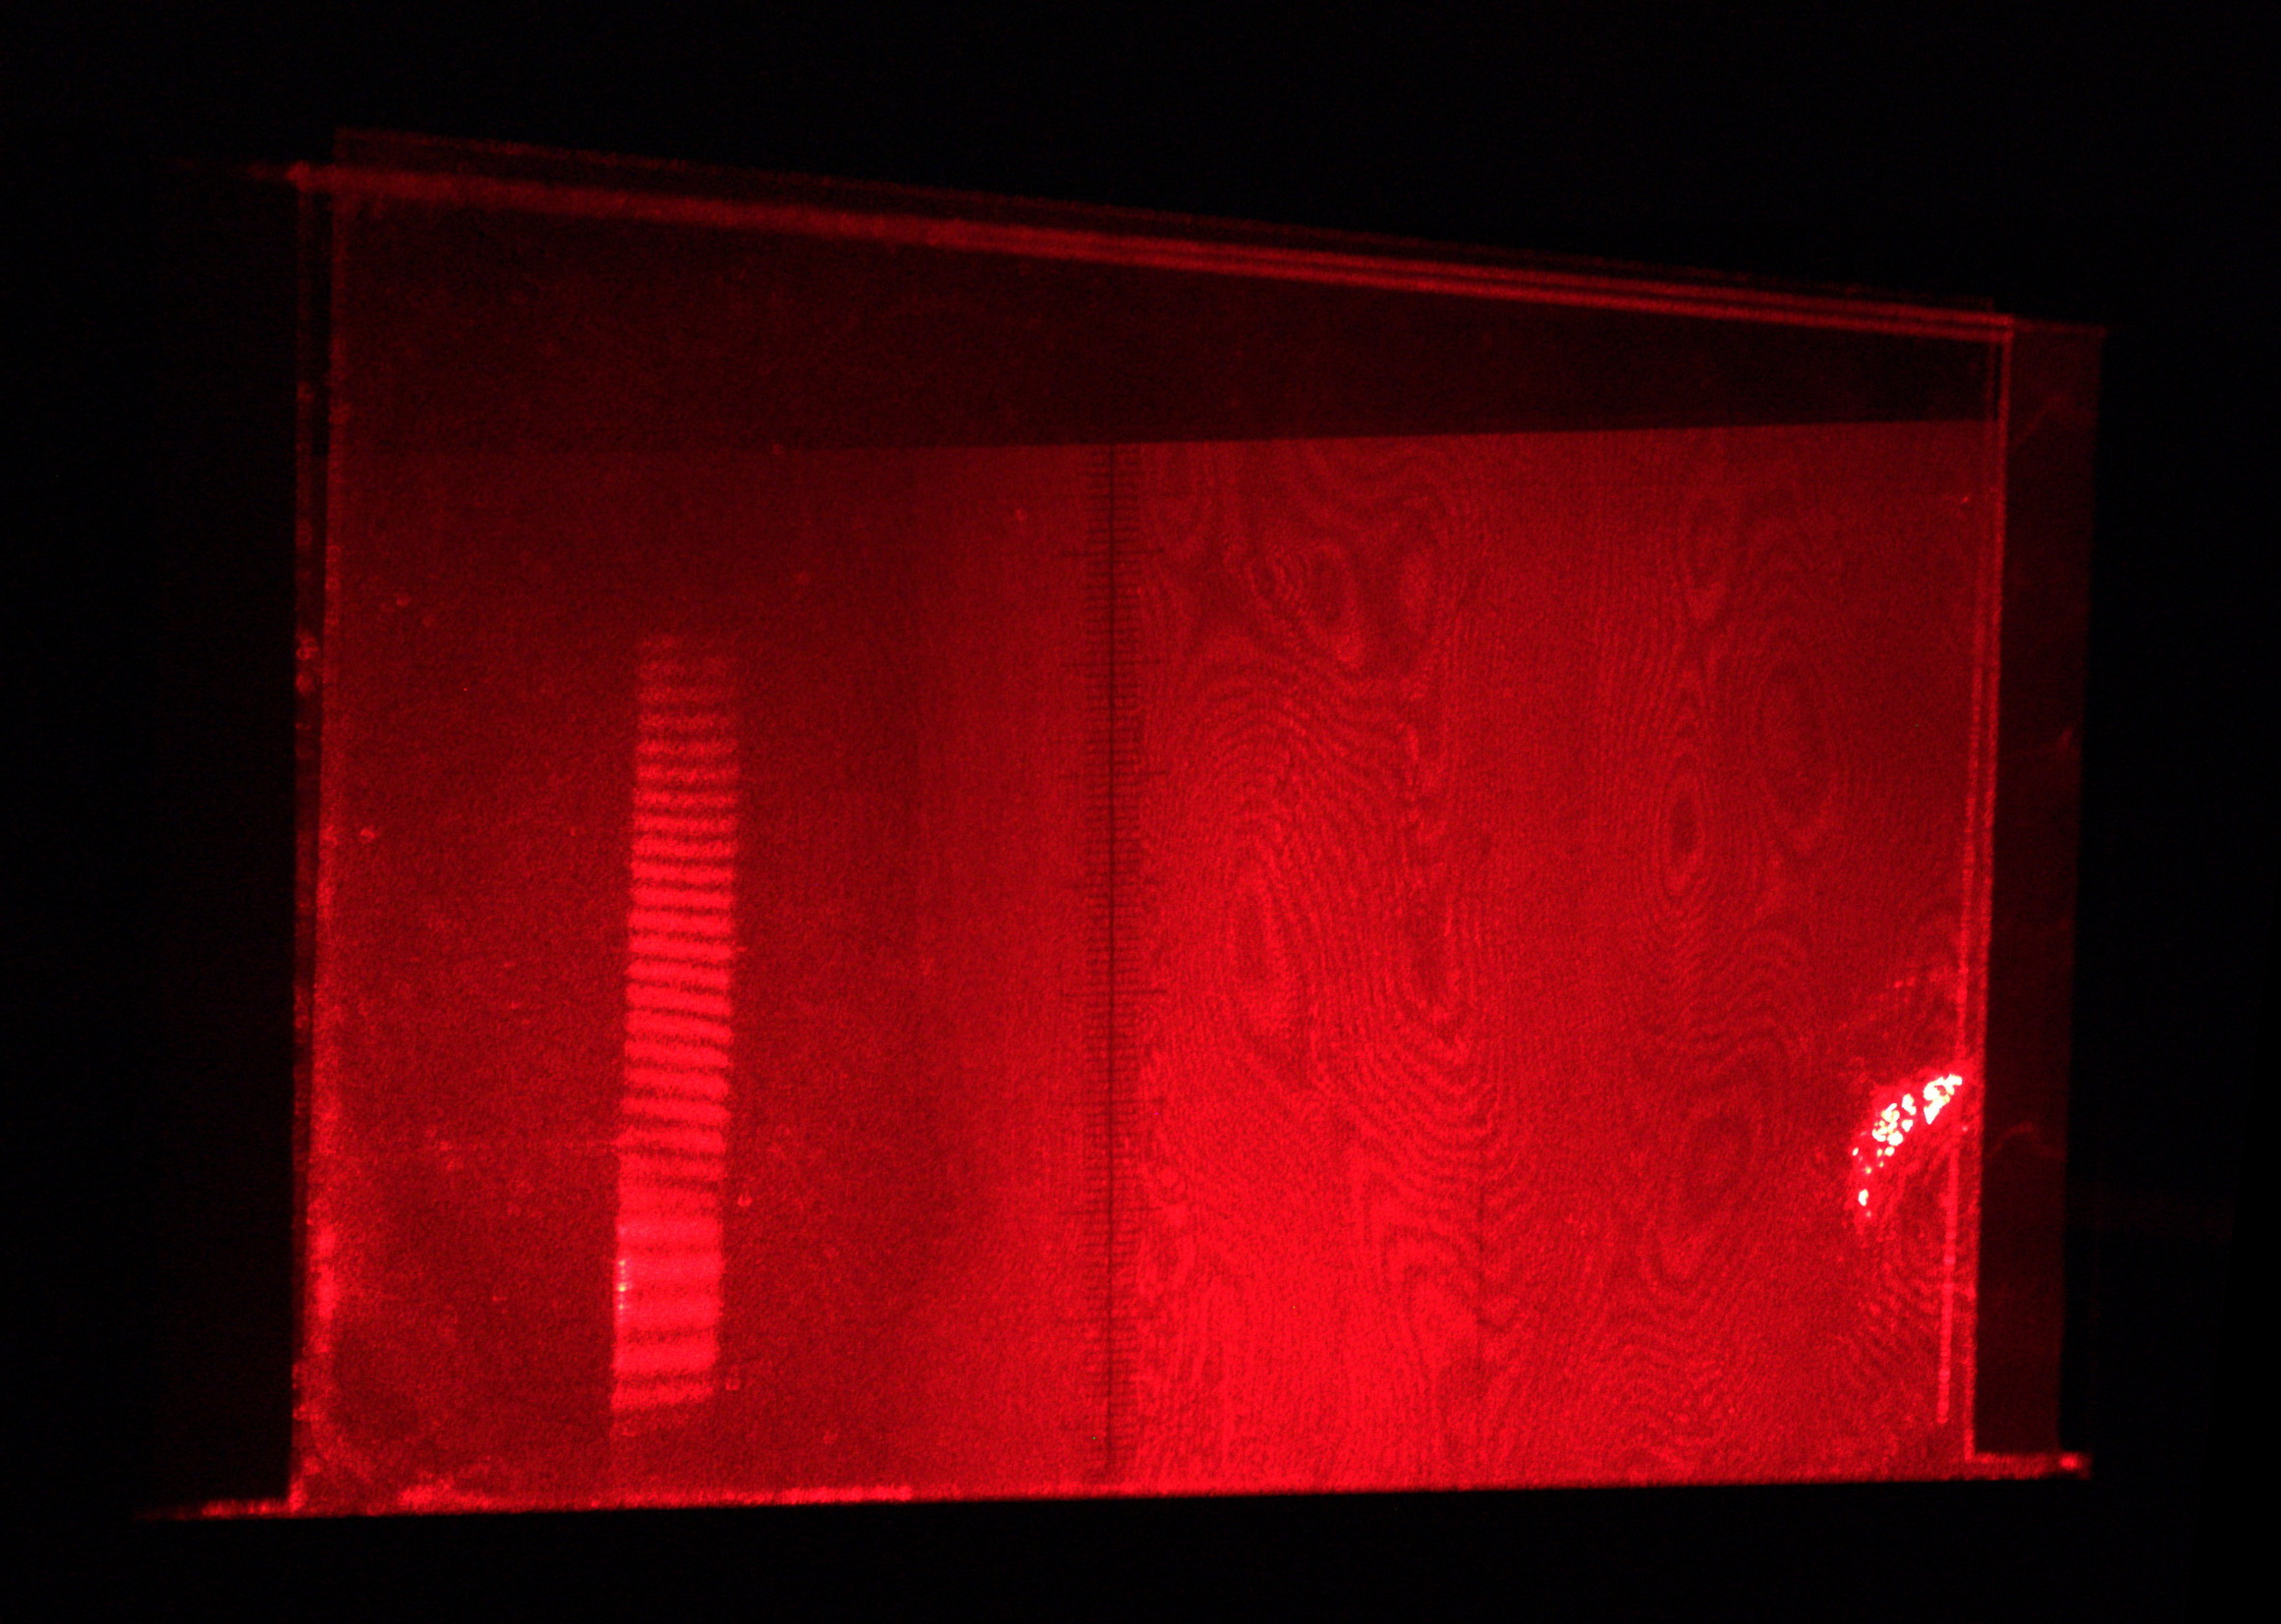
\includegraphics[width=\textwidth]{Photos/IMG_3919-korrigiert.jpg}
 \caption{Hologramm des rechten Stabes mit Perspektivenkorrektur}
 \label{doppelbelichtung-rechts-korrigiert}
\end{figure}
Das erste Minimum des Interferenzmusters ausgehend von der Befestigung entspricht einer Differenz von $\Delta x_1 = \nicefrac{\lambda}{2}$, die weiteren Minimas liegen dann bei $\Delta x_i = \Delta x_{i-1} + \lambda$. Wir haben also eine Perspektivenkorrektur (Abb. \ref{doppelbelichtung-rechts-korrigiert}) vorgenommen und mit dem Programm {\verb Engauge Digitizer} über die Skala des Schirms die Position der Minima abgelesen und die Verbiegung berechnet. 


\begin{figure}[ht]
 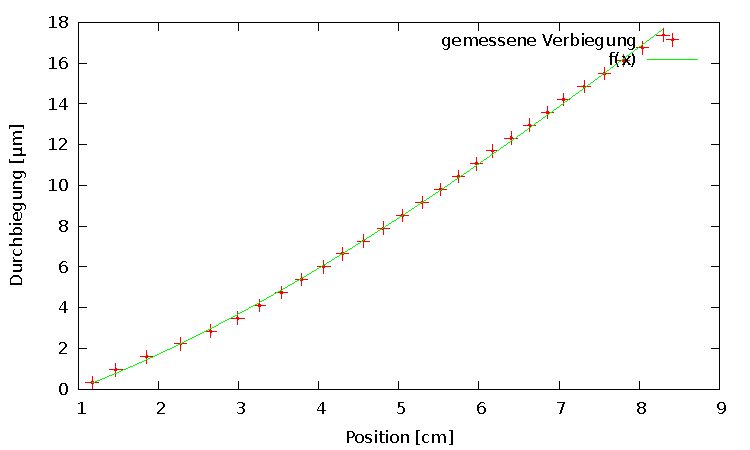
\includegraphics[width=\textwidth]{Graphen/biegung-balken3.pdf}
 \caption{Durchbiegung des Aluminium-Stabes}
\end{figure}

%TODO: ...
